% Template for Cogsci submission with R Markdown

% Stuff changed from original Markdown PLOS Template
\documentclass[10pt, letterpaper]{article}

\usepackage{cogsci}
\usepackage{pslatex}
\usepackage{float}
\usepackage{caption}

% amsmath package, useful for mathematical formulas
\usepackage{amsmath}

% amssymb package, useful for mathematical symbols
\usepackage{amssymb}

% hyperref package, useful for hyperlinks
\usepackage{hyperref}

% graphicx package, useful for including eps and pdf graphics
% include graphics with the command \includegraphics
\usepackage{graphicx}

% Sweave(-like)
\usepackage{fancyvrb}
\DefineVerbatimEnvironment{Sinput}{Verbatim}{fontshape=sl}
\DefineVerbatimEnvironment{Soutput}{Verbatim}{}
\DefineVerbatimEnvironment{Scode}{Verbatim}{fontshape=sl}
\newenvironment{Schunk}{}{}
\DefineVerbatimEnvironment{Code}{Verbatim}{}
\DefineVerbatimEnvironment{CodeInput}{Verbatim}{fontshape=sl}
\DefineVerbatimEnvironment{CodeOutput}{Verbatim}{}
\newenvironment{CodeChunk}{}{}

% cite package, to clean up citations in the main text. Do not remove.
\usepackage{cite}

\usepackage{color}

% Use doublespacing - comment out for single spacing
%\usepackage{setspace}
%\doublespacing


% % Text layout
% \topmargin 0.0cm
% \oddsidemargin 0.5cm
% \evensidemargin 0.5cm
% \textwidth 16cm
% \textheight 21cm

\title{Predicting Age of Acquisition for Early Words Across Languages}


\author{{\large \bf Mika Braginsky} \\ \texttt{mikabr@stanford.edu} \\ Department of Psychology \\ Stanford University \And {\large \bf Daniel Yurovsky} \\ \texttt{yurovsky@stanford.edu} \\ Department of Psychology \\ Stanford University \And {\large \bf Virginia A. Marchman} \\ \texttt{marchman@stanford.edu} \\ Department of Psychology \\ Stanford University \And {\large \bf Michael C. Frank} \\ \texttt{mcfrank@stanford.edu} \\ Department of Psychology \\ Stanford University}

\begin{document}

\maketitle

\begin{abstract}
\emph{{[}TODO: abstract{]}}

\textbf{Keywords:}
language acquisition; word learning; development
\end{abstract}

\section{Introduction}\label{introduction}

One of the central problems facing a child acquiring their first
language is to learn word meanings -- figuring out how to map the
wordforms they hear onto representations of their meanings, in the face
of noisy input and uncertainty about the speaker's intended referent for
any word. \emph{{[}TODO: this doesn't feel like a neutral enough framing
of the problem but I'm not sure how to make it better; it also feels
like more of some sort of broad motivation is needed{]}}

Researchers have proposed a number of strategies that learners could be
using to tackle this problem, each of which has accumulated substantial
experimental evidence of its plausibility: young children seem to track
co-occurence statistics between words and referents to deduce word
meaning across situations; they seem to attend to social cues like
pointing and eye gaze to direct their hypothesis search; they seem to be
equipped with certain biases, such as priviledging basic level category
labels, constraining their inference; they seem to draw on their
knowledge of relations between words to use known meaning to learn new
ones; and so on. \emph{{[}TODO: citations for each thing{]}} While each
of these abilities has been reliably demonstrated in constrained
learning contexts in the laboratory, it is less clear to what extent
children employ them in the natural word learning environment and how
they interact to create the longer-term dynamics of vocabulary
acquisition. How do various word learning mechanisms differ in their
relative contributions, and how does that change over the course of
development?

To disentangle these factors within the real-world word leaning setting,
we can look across children to determine how easy or hard various words
are to learn, and then examine the relationship between words'
difficulties and various word properties that relate to proposed word
learning mechanisms. Foundational work using such an approach has
revealed that in English, within lexical category, words that are more
frequent in speech to children are likely to be learned earlier
(Goodman, Dale, \& Li, 2008). More recently, English and Spanish words'
iconocity, the degree to which their form resembles their meaning, has
been found to relate to age of acquisition (Perry, Perlman, \& Lupyan,
2015). \emph{{[}TODO: what work is missing from this summary?{]}}.
However, previous studies have focused on examining an individual
factor, making it difficult to compare the relative importance of the
many factors known or hypothesized to contribute to word learning. To
more thoroughly investigate the question of what properties determine
words' learnability, our study incorporates a variety of
theoretically-important factors, as well as basing our analysis on a
large samples of words and children, and building towards more
cross-linguistic coverage.

We conduct such an analysis by using parent-report data from the
MacArthur-Bates Communicative Development Inventory (CDI) to estimate
the age of acquisition (AoA) for around 400 words in each of 7
languages. We also use the CHILDES database to estimate each words'
frequency and mean length of utterances (MLU) in which it appears, as
well as obtaining ratings of each words' concreteness, valence, arousal,
and relevance to babies from previously collected norms. We then predict
words' AoA from all of these properties, and assess the relative
contributions of each factor, along with the interaction of predictors
with the lexical category and their changes over development.

\emph{{[}TODO: need to relate predictors to theories, at least vaguely,
not sure how to do this without setting up strawmen{]}}

\emph{{[}TODO: something about how this whole thing will help understand
mechanisms of word learning{]}}

\newpage

\section{Methods}\label{methods}

We use Wordbank (wordbank.stanford.edu), an open database of
developmental vocabulary data, to estimate the age of acquisition for
words across 7 languages: English, Italian, Norwegian, Russian, Spanish,
Swedish, Turkish. We then ask what factors are most important for
predicting this age of acquisition.

\subsection{Estimating AoA}\label{estimating-aoa}

To estimate the age at which words are acquired, we took vocabulary data
collected using the MacArthur-Bates Communicative Development Inventory,
a family of parent-report checklists (Fenson, 2007), specifically the
Words \& Gestures (infant) form for 8- to 18-month-olds. When filling
out a CDI a form, parents are asked to indicate whether their child
understands and/or says each of around 400 words. From these data, for
each word on the CDI, we computed the proportion of children at each age
that are reported to understand the word. We then fit a logistic curve
to these proportions and determine when the curve crosses 0.5, i.e.~at
what age at least 50\% of children are reported to understand the word.
This point is taken to be the words' age of acquisition.

\subsection{Predictors}\label{predictors}

Each of our predictors are derived from independent resources. For each
word that appears on the CDI Word \& Gestures form in each of our 7
languages, we obtained an estimate of its frequency in child-directed
speech, the mean utterance length (MLU) of sentences in which if appears
in child-directed speech, its length in characters, and ratings of its
concreteness, valence, arousal, and relevance to babies. While frequency
and MLU are measured relative to the word's language, since the
conceptual ratings were collected only in English, we mapped all the
words onto translation equivalents across CDI forms, allowing us to use
the ratings for English words cross-linguistically. While imperfect,
this method allows us to examine languages for which limited resources
exist.

Items such as \emph{child's own name} were excluded in all languages.
Each predictor was also centered and scaled so that they would all have
comparable units.

\textbf{Frequency}: For each language, we estimated word frequency from
unigram count in all corpora in the CHILDES database (MacWhinney, 2000)
for that language, normalized to the length of the corpus. Each word's
count includes the counts of words that share the same stem (so that
\emph{dogs} counts as \emph{dog}) or are synonymous (so that
\emph{father} counts as \emph{daddy}). For polysemous word pairs, such
as \emph{orange} as in color and \emph{orange} as in fruit, each
occurence of \emph{orange} in the corpus counts for both. Finally, each
word's frequency estimate is taken as the log of its count.

\textbf{MLU}: For each language, we estimated each word's MLU by
calculating the mean number of words in the sentences in which that word
appears in all corpora in the CHILDES database for that language. Words
that only occur in one sentence were excluded \emph{{[}TODO: do this
exclusion{]}}.

\textbf{Length}: We computed the number of characters in each word in
each language, which is known to be highly correlated with number of
phonemes and syllables.

\textbf{Concreteness}: We used previously collected norms for
concreteness (Brysbaert, Warriner, \& Kuperman, 2014), which were
gathered by asking adult participants to rate how concrete the meaning
of each word is by using a 5-point scale from abstract to concrete. For
the 10 CDI words that weren't part of the collected norms (mostly animal
sounds such as \emph{baa baa}), we imputed a conreteness rating from the
mean of all CDI words' concreteness rating.

\textbf{Valence and Arousal}: We also used previously collected norms
for valence and arousal (Warriner, Kuperman, \& Brysbaert, 2013), for
which adult participants are asked to rate words on a 1-9 happy-unhappy
scale (valence) and 1-9 excited-calm scale (arousal). For the 43 CDI
words that weren't part of the collected norms (mostly function words
such as \emph{her}), we imputed ratings from the mean of all CDI words'
ratings.

\textbf{Babiness}: Lastly, we used previously collected norms of
``babiness'', a measure of association with infancy (Perry et al., 2015)
for which adult participants are asked to judge how relevant to babies a
word is.

\section{Analysis}\label{analysis}

We present three analyses of these data: 1) how the word properties
change over development, 2) their relative contributions to predicting
AoA, and 3) their interaction with lexical category.

\subsection{Developmental Trajectory}\label{developmental-trajectory}

To assess developmental trends, we examine how the values of each
predictor change as a function of estimated AoA. Figure \ref{fig:devo}
shows these trajectories averaged over all words. Words that are learned
earlier are more frequent, higher in babiness, and appear in shorter
sentences. Concreteness exhibits a U-shaped trajectory, with the
earliest learned words actually being relatively abstract, since many
are social routines and animal sounds. \emph{{[}TODO: statistical tests?
better model than loess? more compelling presentation?{]}}

\begin{CodeChunk}
\begin{figure*}[tb]

{\centering 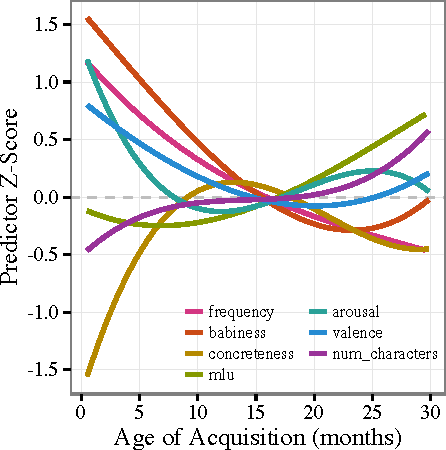
\includegraphics{figs/devo-1} 

}

\caption[Predictor values over development]{Predictor values over development.}\label{fig:devo}
\end{figure*}
\end{CodeChunk}

\newpage

\subsection{Predicting AoA}\label{predicting-aoa}

We fit a linear regression for each language's data, as well as a linear
mixed-effects model with language as a random effect for all the data
pooled. Figure \ref{fig:coefs} shows the magnitude of the coefficient
for each predictor in each language and cross-linguistically. We find
that frequency, concreteness, and babiness are relatively stronger
predictors of age of acquisition, across languages and in the
cross-linguistic model. \emph{{[}TODO: say stuff about significance of
coefs? say more other stuff?{]}}

\begin{CodeChunk}
\begin{figure*}[tb]

{\centering 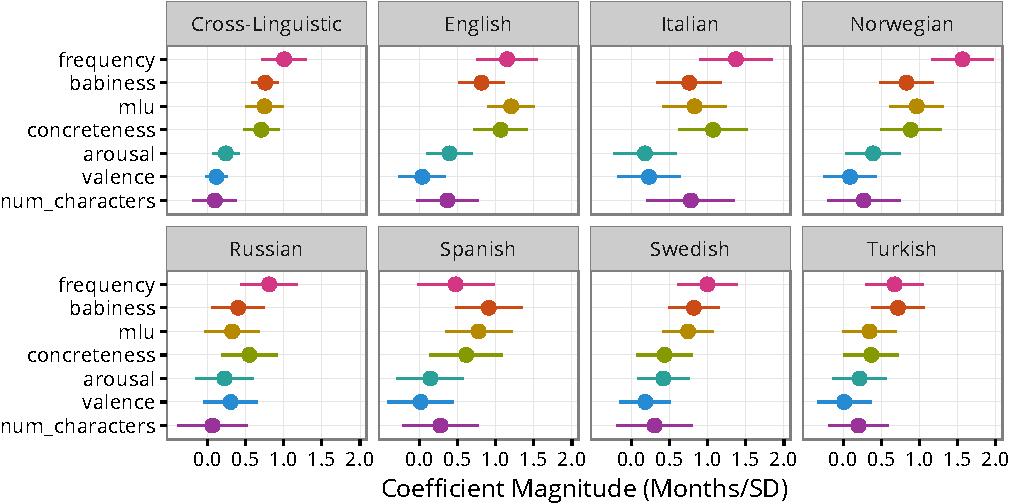
\includegraphics{figs/coefs-1} 

}

\caption[Magnitudes of predictor coefficients]{Magnitudes of predictor coefficients.}\label{fig:coefs}
\end{figure*}
\end{CodeChunk}

\subsection{Lexical Category}\label{lexical-category}

\emph{{[}TODO: no idea how to do this whole analysis
properly\ldots{}{]}}

\begin{CodeChunk}
\begin{figure*}[tb]

{\centering 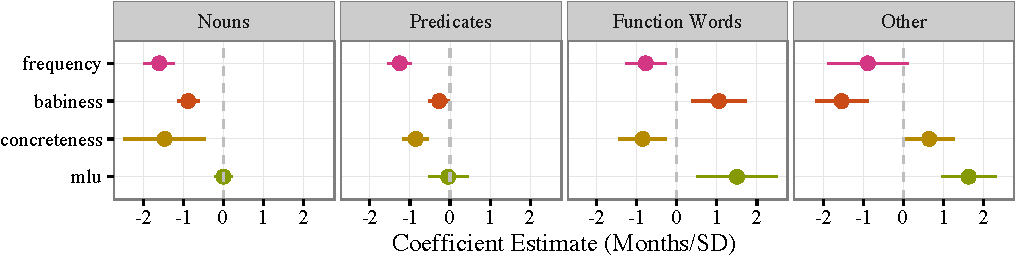
\includegraphics{figs/coefs_lexcat-1} 

}

\caption[Magnitudes of predictor coefficients by lexical category]{Magnitudes of predictor coefficients by lexical category.}\label{fig:coefs_lexcat}
\end{figure*}
\end{CodeChunk}

\newpage

\section{Discussion}\label{discussion}

Overall, we find that while frequency is predictive of age of
acquisition across languages, conceptual factors are at least as
important, especially for the earliest learned words. Our results imply
that distributional theories of word learning should be constrained by
such conceptual factors, which are likely to apply across languages.
\emph{{[}TODO: actually say something{]}}

\newpage

\section{Conclusion}\label{conclusion}

\emph{{[}TODO: say some more things{]}}

\section{Acknowledgements}\label{acknowledgements}

Thanks to the MacArthur-Bates CDI Advisory Board.

\section{References}\label{references}

\setlength{\parindent}{-0.1in} \setlength{\leftskip}{0.125in} \noindent

Brysbaert, M., Warriner, A. B., \& Kuperman, V. (2014). Concreteness
ratings for 40 thousand generally known english word lemmas.
\emph{Behavior Research Methods}, \emph{46}(3), 904--911.

Fenson, L. (2007). \emph{MacArthur-bates communicative development
inventories: User's guide and technical manual}. Paul H. Brookes
Publishing Company.

Goodman, J. C., Dale, P. S., \& Li, P. (2008). Does frequency count?
Parental input and the acquisition of vocabulary. \emph{Journal of Child
Language}, \emph{35}(3), 515.

MacWhinney, B. (2000). \emph{The cHILDES project: The database} (Vol.
2). Psychology Press.

Perry, L. K., Perlman, M., \& Lupyan, G. (2015). Iconicity in english
and spanish and its relation to lexical category and age of acquisition.
\emph{PloS One}, \emph{10}(9), e0137147.

Warriner, A. B., Kuperman, V., \& Brysbaert, M. (2013). Norms of
valence, arousal, and dominance for 13,915 english lemmas.
\emph{Behavior Research Methods}, \emph{45}(4), 1191--1207.

\end{document}
